\section{真値条件の悪化の詳細}\label{sup:projection}
\begin{figure}[tbp]
  \centering
  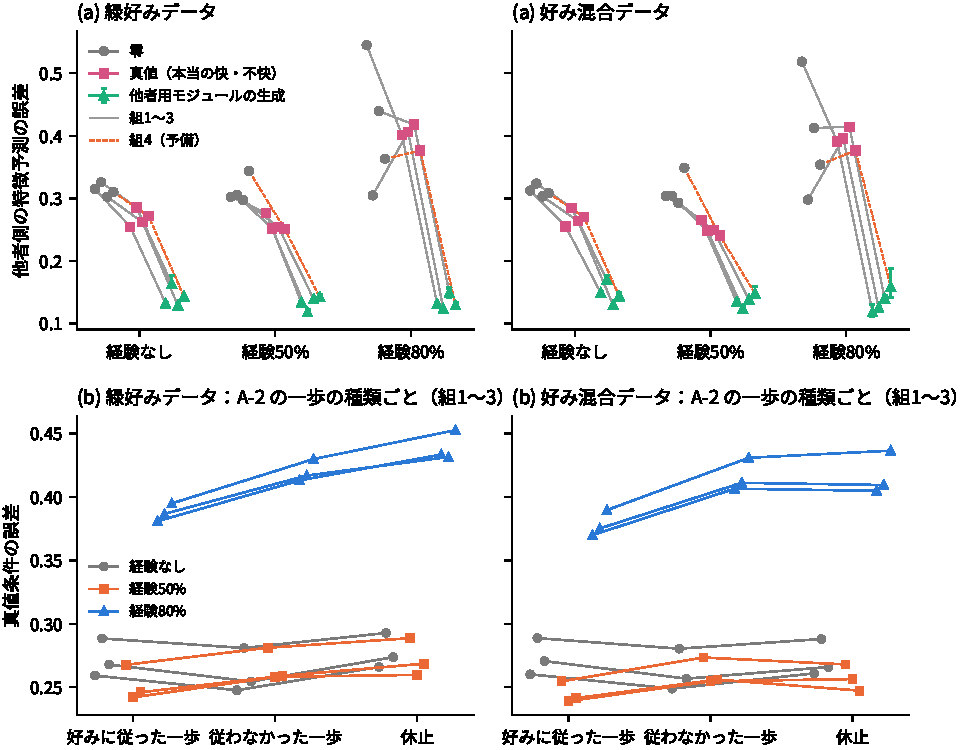
\includegraphics[width=\linewidth]{figs/projection_error}
  % 図4：投影の誤り（実験2の真値条件）。他者側の特徴予測の誤差を，process-2 に零・本当の快・不快（D6）・
  % 他者用モジュールが生成した Q2 を入れた3通りで，経験なし・50%・80% ごとに組別に並べる（組1〜3，組4 があれば足す）。
  % ログに一歩の種類ごとの集計があれば (b) として足す。
  % 元：v13 のログ・まとめの真値条件（T3・D6）の節（Claude Code が README に書く）。
  \caption{他者の本当の快・不快を与えたときの他者側の特徴予測の誤差．(a)(b) 緑好みデータと好み混合データで，process-2 に零，本当の快・不快，他者用モジュールの出力を入れた場合を，経験の量ごとに示す（組1〜3 は灰の実線，組4 は橙の破線）．(c)(d) 本当の快・不快を入れた場合の誤差を，A-2 の一歩の種類（好みに従った一歩，従わなかった一歩，休止）ごとに示す（組1〜3）．}
  \label{fig:projection}
\end{figure}

\begin{table}[tbp]
  \centering
  \small
  \caption{真値条件における他者側の特徴予測の誤差}
  \label{tab:projection}
  % paper/tables/projection.tex -- generated by analyze/paper/tables_paper.py; sources in paper/tables/README.md
\begin{tabular}{@{}lllllll@{}}
\toprule
 & \multicolumn{3}{l}{緑好みデータ} & \multicolumn{3}{l}{好み混合データ} \\
\cmidrule(lr){2-4}\cmidrule(l){5-7}
条件・組 & 零 & 真値 & 生成 & 零 & 真値 & 生成 \\
\midrule
経験なし・組1 & 0.315 & 0.255 & 0.131〜0.134 & 0.313 & 0.255 & 0.146〜0.151 \\
経験なし・組2 & 0.326 & 0.286 & 0.159〜0.176 & 0.324 & 0.285 & 0.167〜0.177 \\
経験なし・組3 & 0.302 & 0.262 & 0.125〜0.132 & 0.303 & 0.264 & 0.128〜0.131 \\
経験なし・組4 & 0.310 & 0.271 & 0.141〜0.145 & 0.308 & 0.270 & 0.142〜0.149 \\
\midrule
経験50\%・組1 & 0.302 & 0.276 & 0.132〜0.135 & 0.304 & 0.265 & 0.133〜0.138 \\
経験50\%・組2 & 0.305 & 0.252 & 0.116〜0.122 & 0.304 & 0.248 & 0.121〜0.127 \\
経験50\%・組3 & 0.297 & 0.254 & 0.138〜0.142 & 0.293 & 0.249 & 0.138〜0.139 \\
経験50\%・組4 & 0.344 & 0.252 & 0.140〜0.146 & 0.349 & 0.241 & 0.143〜0.159 \\
\midrule
経験80\%・組1 & 0.545 & 0.402 & 0.129〜0.133 & 0.519 & 0.391 & 0.112〜0.130 \\
経験80\%・組2 & 0.305 & 0.406 & 0.121〜0.126 & 0.298 & 0.396 & 0.123〜0.127 \\
経験80\%・組3 & 0.440 & 0.418 & 0.142〜0.157 & 0.413 & 0.414 & 0.134〜0.145 \\
経験80\%・組4 & 0.363 & 0.376 & 0.126〜0.134 & 0.354 & 0.377 & 0.141〜0.188 \\
\midrule[\heavyrulewidth]
\multicolumn{7}{@{}l}{真値条件の誤差を A-2 の一歩の種類で分けたもの（組1〜3 の範囲．括弧は一歩のうちその種類の割合）} \\
\midrule
データ・一歩 & \multicolumn{2}{l}{経験なし} & \multicolumn{2}{l}{経験50\%} & \multicolumn{2}{l}{経験80\%} \\
\midrule
緑好み・好みに従った一歩（0.43） & \multicolumn{2}{l}{0.259〜0.289} & \multicolumn{2}{l}{0.242〜0.268} & \multicolumn{2}{l}{0.381〜0.395} \\
緑好み・従わなかった一歩（0.49） & \multicolumn{2}{l}{0.248〜0.281} & \multicolumn{2}{l}{0.258〜0.281} & \multicolumn{2}{l}{0.413〜0.430} \\
緑好み・休止（0.08） & \multicolumn{2}{l}{0.266〜0.293} & \multicolumn{2}{l}{0.260〜0.289} & \multicolumn{2}{l}{0.432〜0.453} \\
好み混合・好みに従った一歩（0.42） & \multicolumn{2}{l}{0.260〜0.289} & \multicolumn{2}{l}{0.239〜0.255} & \multicolumn{2}{l}{0.370〜0.390} \\
好み混合・従わなかった一歩（0.49） & \multicolumn{2}{l}{0.249〜0.280} & \multicolumn{2}{l}{0.255〜0.273} & \multicolumn{2}{l}{0.407〜0.431} \\
好み混合・休止（0.09） & \multicolumn{2}{l}{0.261〜0.288} & \multicolumn{2}{l}{0.247〜0.268} & \multicolumn{2}{l}{0.405〜0.437} \\
\bottomrule
\end{tabular}

  % 表4：零・真値（D6）・生成した Q2 の誤差を，経験なし・50%・80% ごと，組ごと。
  % 一歩の種類ごとの集計がログにあれば，その行を足す。出典：v13 まとめ §4，v13 ログ §24・§25。
\end{table}

A-2 の本当の快・不快を process-2 に入れたときの他者側の予測の誤差は，経験80\%条件で大きくなり，経験の少ない条件より外れた（図\ref{fig:projection}，表\ref{tab:projection}．経験80\%条件では，段階IIを行った4組のうち2〜3組で，何も与えない場合より悪かった）．
真値条件の他者側の特徴予測の誤差は，段階IIを行った組1〜4 と二つのデータを通して，経験なし条件 0.25〜0.29，経験50\%条件 0.24〜0.28 であったのに対し，経験80\%条件では 0.38〜0.42 であった（表\ref{tab:projection}）．
経験なし条件と経験50\%条件の値はほぼ同じで，大きくなったのは経験80\%条件である．
経験80\%条件で，本当の快・不快を入れた方が何も与えない場合（零を入れた場合）より誤差が大きかったのは，緑好みデータで組2・組4 の2組，好み混合データで組2〜4 の3組であった（追加の比較で測った全6組では，それぞれ3組と4組）．
% 出典：numbers_check.md（Claude Code 第2弾。好み混合の組3：真値 0.4141 対 零 0.4127）。
% 出典：v13 まとめ §4（組1〜3），組4（経験なし 0.272，50% 0.252，80% 0.377，零 0.363）は Claude Code 第1弾の報告と tables/projection.tex。
% 組5・6 は段階IIを行っていないので値がない。
この悪化は予想していなかった結果である．

悪化の大部分は，A-2 がどう動いたかによらない予測の中の位置のずれであると読める（事後の分析による推測）．
経験80\%条件と経験50\%条件の差は，A-2 が好みに従って動いた一歩でも $+0.11$〜$+0.15$ あり，好みに従わなかった一歩や休止の一歩ではそれよりやや大きかった（3組で同じ順．図\ref{fig:projection}(c)(d)）．
% 出典：v13 まとめ §4（「悪化は A-2 が好みに従った一歩でも +0.11〜+0.15 あり，従わなかった一歩・眠りでやや大きい（+0.01〜+0.04，「従った < 従わなかった < 眠り」の順で 3 組そろう）」）。
%   +0.11〜+0.15 が「80%−50%」の差か，+0.01〜+0.04 が何と何の差かは v13 ログ §24・§25 で【要確認】。
また，快・不快を保つ前の時点で，経験80\%条件のモデルは予測の中の A-2 を本当の位置より A-2 の好きな色の方へ寄せて置いていた（$+0.5$〜$+3.7$．経験50\%条件では逆に $-0.7$〜$-1.9$）．
% 出典：v13 まとめ §3.1 の表（止める前の A-2 の置き方。事後の分析）。
経験80\%条件の A-1 は，快が高ければほぼ好きな色の角にいた．
一つの解釈は，その経験から，モデルが他者を自分と同じ強さで快の方へ動く者として見積もり，半分しか好みに従わない A-2 を本当より快の方へ寄せて予測したというものである（自分の行動の仕方の投影）．
寄せる向きは，入れた快・不快の正の向き（A-2 の好きな色）であり，A-1 自身の好きな色ではない．
A-1 自身の好きな色への寄りは，調べた範囲（経験50\%条件のモデルと\ref{app:switch}節の好み切替条件）では見られなかった．
% 出典：執筆メモ §5 主張3（v12・v14-C で A-1 自身の好きな色への投影なし），v14 まとめ §3。

ただし，この解釈のほかにも説明が残る．
第一に，段階Iの process-2 には零しか入らないので，本当の快・不快は段階Iのモデルにとって学習で見ていない入力である．
もっとも，同じ入力を入れた経験なし条件と経験50\%条件では誤差は 0.24〜0.29 にとどまり，経験50\%条件では零を入れるよりやや小さかった（零で約 0.30〜0.35）．
したがって，見ていない入力であることだけでは条件の違いを説明できないが，見ていない入力への応じ方が経験の量によって変わった可能性は残る．
第二に，経験80\%条件の学習データの位置の偏りそのものが，他者の位置の予測を角の方へ寄せた可能性がある．
これは自分の行動の仕方の投影と近いが，価値に従って動いた経験ではなく，角に多くいた経験から生じる点で区別される．
評価は全条件で同じデータを用いたので，評価の場面の違いによる説明は当たらない．

\paragraph{他者の行動の仕方を自分にそろえた比較}
そこで，A-2 も 0.8 の割合で好みに従う評価用データで同じ比較を行った（本文3.4節，本文の図4）．
事前登録した三つの予想は，緑好みデータと好み混合データの両方で，本番の3組すべてと全6組すべてで成り立った．
第一に，経験80\%条件では，A-2 の割合を 0.5 から 0.8 にすると $\Delta$ が小さくなった（本当の快・不快がより役立った）．組をまたいだ変化は，緑好みデータで $-0.096$ [$-0.139$, $-0.054$]，好み混合データで $-0.098$ [$-0.125$, $-0.071$] であった．
第二に，この変化は経験50\%条件より経験80\%条件で大きかった（交互作用 $-0.056$ [$-0.100$, $-0.012$]，$-0.046$ [$-0.072$, $-0.020$]）．
第三に，経験80\%条件と経験なし条件の間の交互作用も同じ向きであった（$-0.071$ [$-0.112$, $-0.030$]，$-0.071$ [$-0.101$, $-0.040$]）．
% 出典：paper_extra_results_log.md（A1・A2・A3，全6組の t の 95% CI，自由度5）。
ただし，A-2 を 0.8 にすると，どの条件でも本当の快・不快はいくらか役立つようになった（A-2 の割合を 0.5 から 0.8 にしたときの $\Delta$ の変化は，組1〜6 と二つのデータを通して，経験なし条件で $-0.016$〜$-0.036$，経験50\%条件で $-0.035$〜$-0.059$，経験80\%条件で $-0.05$〜$-0.16$）．
% 確認：Δ の変化（A-2 0.8 − 0.5）。組ごとの値は paper_extra_results_log.md §A.1・§A.2 の「対比」の表（D_なし・D_50・D_A1）。
また，悪化は消えたのではなく小さくなった．A-2 が 0.8 のとき，経験80\%条件と経験50\%条件の差は，組1・組3 では逆になり（経験80\%条件の方が役立つ），組2・組4・組5 では経験80\%条件の方がまだ悪いが差は小さくなり，組6 では好み混合データで0前後，緑好みデータではまだ悪かった（$+0.032$ [$+0.017$, $+0.047$]）．
また組2 では，A-2 が 0.8 のときにも経験80\%条件で本当の快・不快が零より悪いままであった．
% 出典：numbers_check.md #8・#10（paper_extra_results_log.md §A）。
なお，組1 では A-2 が 0.5 のときにも経験80\%条件で本当の快・不快の方が零より良く，既存の悪化の形は再現されないが，三つの予想の向きは組1 でも成り立った．

この結果は，真値条件の悪化が，自分と他者の行動の仕方の食い違いによって大きく変わることを示す．
学習で見ていない入力であることはどの組み合わせでも同じなので，見ていない入力への不安定さだけでは，この違いを説明できない．
一方，A-2 を 0.8 にすると，A-2 も経験80\%条件の A-1 の学習データと同じく，好きな色の角への滞在が増える（後半のフレームで好きな色から距離5未満にいる割合は，A-2 で 0.99〜1.00，経験80\%条件の A-1 の学習データで 0.99）．
位置の分布が全体として一致することまでは確かめていない．
したがってこの比較では，価値に従って動いた経験の投影と，角に多くいた経験による位置の偏りとは分けられない．
位置の分布をそろえた対照でも，この悪化の原因は判定できなかった（本文4.3節）．
